\documentclass[border=3pt]{standalone}
% Preâmbulo compartilhado pelos diagramas TikZ da aula 6 de IHC (Necessidades e Requisitos)
\usepackage[T1]{fontenc}
\usepackage[utf8]{inputenc}
\usepackage{lmodern}
\usepackage{amsmath}
\usepackage{xcolor}
\usepackage{tikz}
\usetikzlibrary{arrows.meta,angles,quotes,decorations.pathmorphing,calc,
                positioning,shapes.geometric,shapes.misc,backgrounds,fit,
                math}

% Paleta (mesma dos SVGs originais)
% Paleta da disciplina de IHC: acento roxo (#755099), da capa do livro.
% (o nome "dblue" é mantido para não alterar todos os diagramas)
\definecolor{dblue}{HTML}{755099}
\definecolor{dorange}{HTML}{B3541E}
\definecolor{dgreen}{HTML}{4A7C59}
\definecolor{dred}{HTML}{9C4B4B}
\definecolor{dcream}{HTML}{F4F1EA}
\definecolor{dshade}{HTML}{DDD7C9}

% Função gaussiana (não normalizada por padrão de escala visual)
\pgfmathdeclarefunction{gauss}{3}{%
  \pgfmathparse{1/(#3*sqrt(2*pi))*exp(-((#1-#2)^2)/(2*#3^2))}%
}

% Estilos comuns (prefixo d... para não colidir com chaves internas do pgf)
\tikzset{
  >={Stealth[length=2mm]},
  dguide/.style={gray!55, dashed, line width=0.4pt},
  daxis/.style={gray!60, line width=0.7pt, ->},
  dbody/.style={fill=black!3, draw=black!80, line width=1pt},
  dacc/.style={draw=dblue, line width=1pt},
  dlbl/.style={black!55, font=\small},
  dsub/.style={black!45, font=\footnotesize},
  dstate/.style={circle, draw=black!80, fill=dcream, line width=1pt,
                 minimum size=17mm, font=\large, inner sep=1pt},
  dobs/.style={circle, draw=black!80, fill=dshade, line width=1pt,
               minimum size=14mm, font=\large, inner sep=1pt},
  dbox/.style={rounded corners=2pt, draw=black!80, fill=dcream, line width=1pt,
               align=center, inner sep=6pt},
  dop/.style={circle, draw=black!80, fill=white, line width=1pt,
              minimum size=6mm, inner sep=0pt, font=\small},
  dtrans/.style={->, dblue, line width=1pt},
  dmeas/.style={->, dorange, line width=1pt},
  dcurve/.style={line width=1pt, dblue},
  dcurveb/.style={line width=1.4pt, dorange},
}

\begin{document}
\hyphenpenalty=10000 \exhyphenpenalty=10000 \tolerance=9999 \emergencystretch=3em
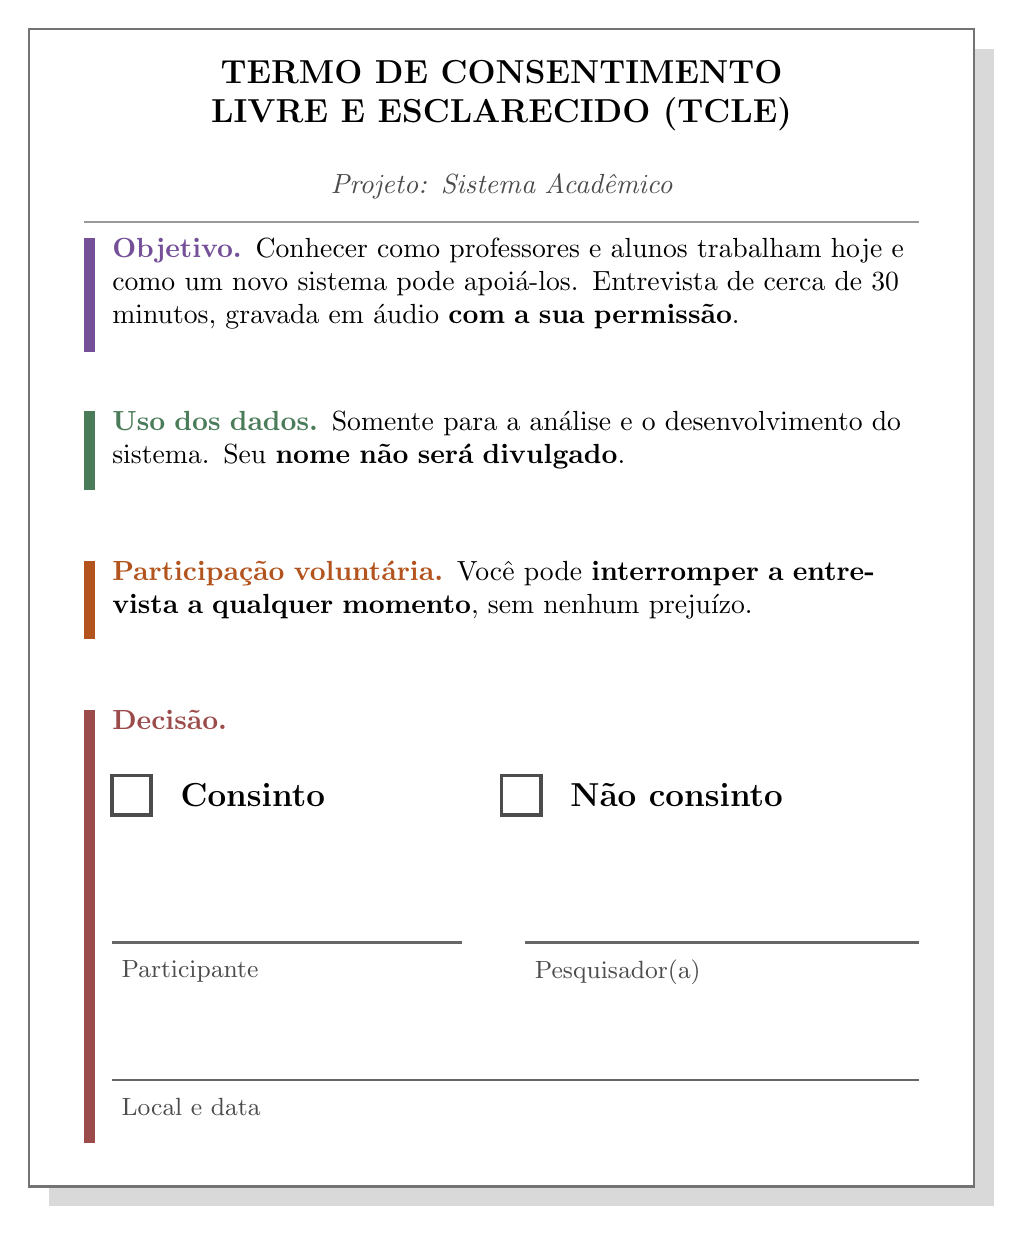
\begin{tikzpicture}[x=1cm,y=1cm]
  \tikzset{sec/.style={anchor=north west, text width=10.1cm, font=\normalsize, align=left, inner sep=0pt}}
  % papel com sombra
  \fill[black!15] (0.25,-0.25) rectangle (12.25,14.45);
  \draw[black!55, fill=white, line width=1pt] (0,0) rectangle (12,14.7);
  % cabeçalho
  \node[font=\large\bfseries, align=center, text width=11cm] at (6,13.85) {TERMO DE CONSENTIMENTO\\ LIVRE E ESCLARECIDO (TCLE)};
  \node[font=\normalsize\itshape, black!70, align=center, text width=11cm] at (6,12.7) {Projeto: Sistema Acadêmico};
  \draw[black!40, line width=0.8pt] (0.7,12.25) -- (11.3,12.25);
  % 1 objetivo
  \fill[dblue] (0.7,10.6) rectangle ++(0.14,1.45);
  \node[sec] at (1.05,12.05) {\textbf{\textcolor{dblue}{Objetivo.}} Conhecer como professores e alunos trabalham hoje e como um novo sistema pode apoiá-los. Entrevista de cerca de 30 minutos, gravada em áudio \textbf{com a sua permissão}.};
  % 2 uso dos dados
  \fill[dgreen] (0.7,8.85) rectangle ++(0.14,1.0);
  \node[sec] at (1.05,9.85) {\textbf{\textcolor{dgreen}{Uso dos dados.}} Somente para a análise e o desenvolvimento do sistema. Seu \textbf{nome não será divulgado}.};
  % 3 participação voluntária
  \fill[dorange] (0.7,6.95) rectangle ++(0.14,1.0);
  \node[sec] at (1.05,7.95) {\textbf{\textcolor{dorange}{Participação voluntária.}} Você pode \textbf{interromper a entrevista a qualquer momento}, sem nenhum prejuízo.};
  % 4 decisão
  \fill[dred] (0.7,0.55) rectangle ++(0.14,5.5);
  \node[sec] at (1.05,6.05) {\textbf{\textcolor{dred}{Decisão.}}};
  \draw[black!70, line width=1.3pt] (1.05,4.72) rectangle ++(0.5,0.5);
  \node[font=\large, anchor=west] at (1.8,4.97) {\textbf{Consinto}};
  \draw[black!70, line width=1.3pt] (6.0,4.72) rectangle ++(0.5,0.5);
  \node[font=\large, anchor=west] at (6.75,4.97) {\textbf{Não consinto}};
  \draw[black!60, line width=0.9pt] (1.05,3.1) -- (5.5,3.1) (6.3,3.1) -- (11.3,3.1);
  \node[font=\small, black!70, anchor=north west] at (1.05,3.0) {Participante};
  \node[font=\small, black!70, anchor=north west] at (6.3,3.0) {Pesquisador(a)};
  \draw[black!60, line width=0.9pt] (1.05,1.35) -- (11.3,1.35);
  \node[font=\small, black!70, anchor=north west] at (1.05,1.25) {Local e data};
\end{tikzpicture}
\end{document}
